\subsubsection{Pruebas del modelo de clasificación}
Como parte del proceso de desarrollo, se realizó una prueba preliminar del modelo de clasificación binaria utilizando EfficientNet-B3 con un subconjunto reducido de datos: 1,500 imágenes por clase (corteza sana y corteza infestada), balanceadas manualmente a partir de los conjuntos disponibles. El objetivo de esta prueba no fue obtener un modelo definitivo, sino validar la viabilidad del enfoque y establecer una línea base para el entrenamiento final.

\begin{figure}[H]
    \centering
    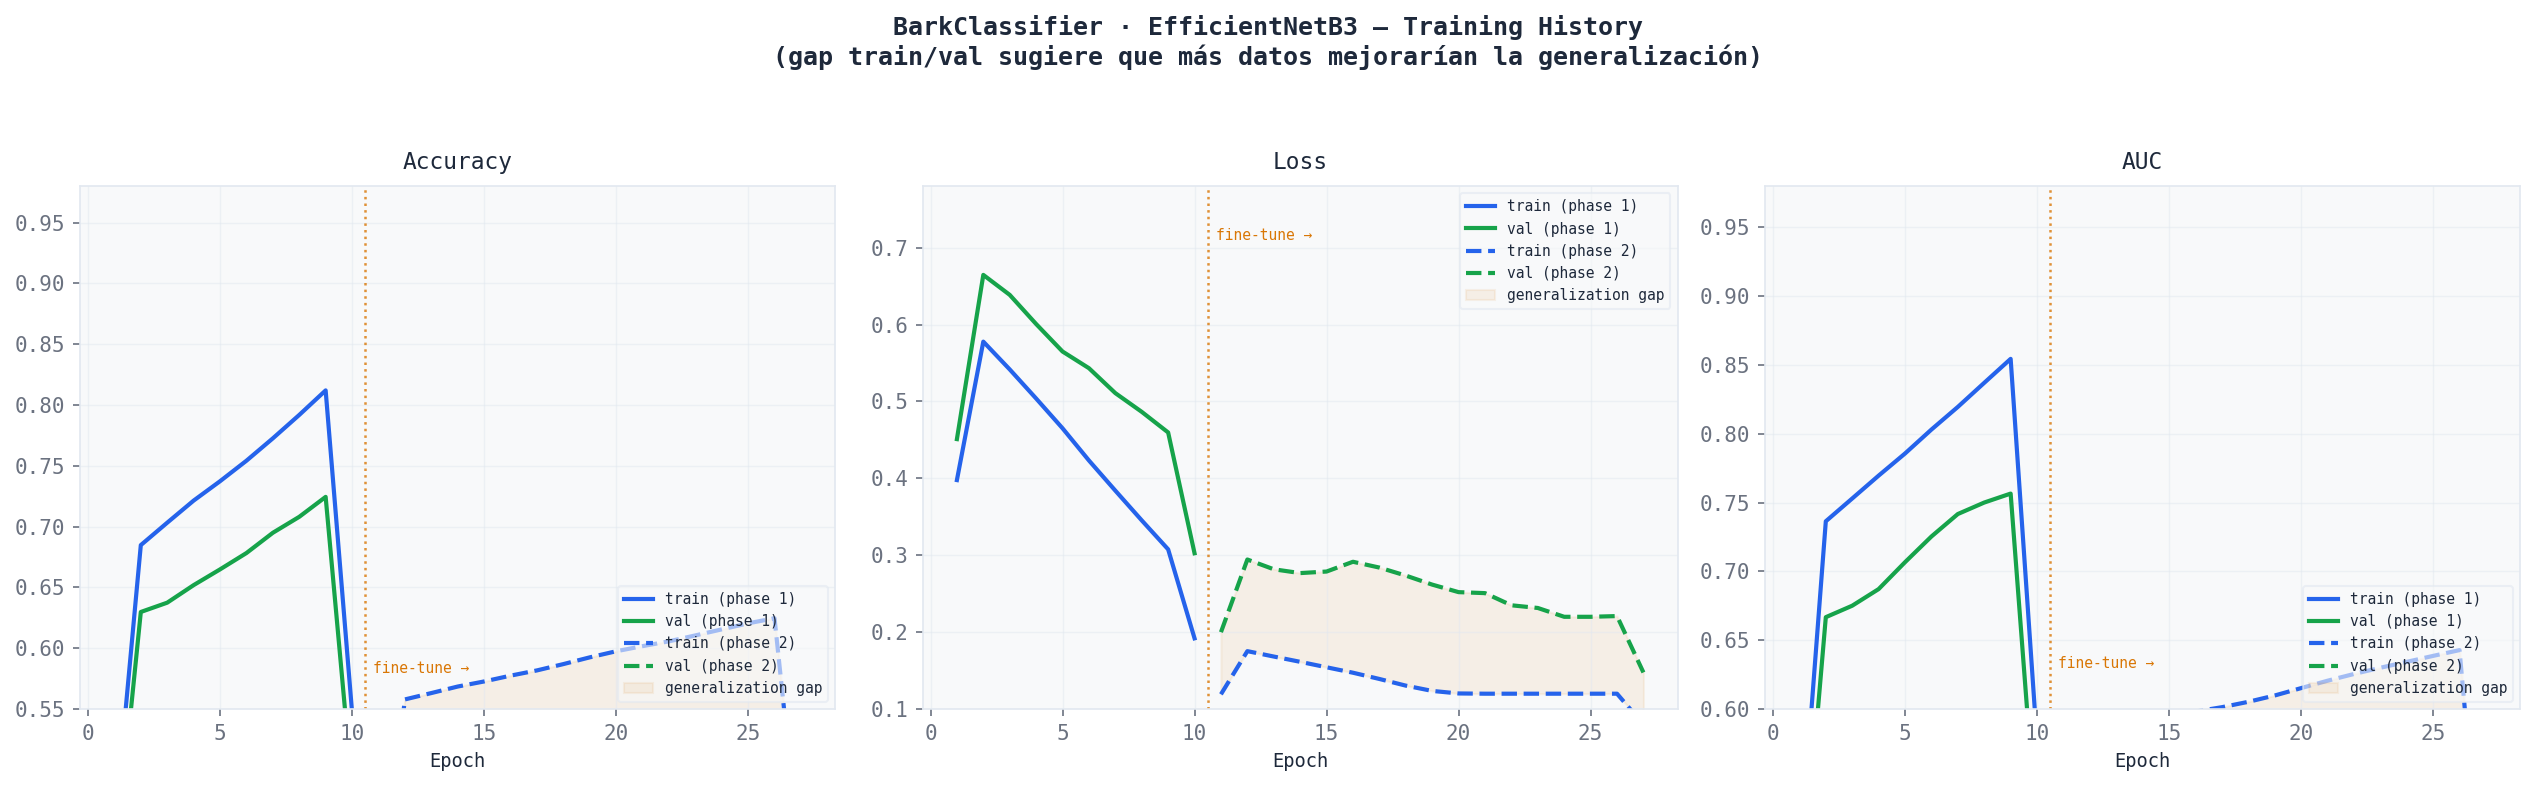
\includegraphics[width=1\textwidth]{images/C7/training_curves.png}
    \caption{Curvas de entrenamiento con dataset de prueba de 1,500 imágenes por clase.}
    \label{fig:training_curves}
\end{figure}

Las curvas de entrenamiento (Figura~\ref{fig:training_curves}) muestran un comportamiento prometedor: la exactitud y el AUC del conjunto de entrenamiento mejoran de forma sostenida a lo largo de las dos fases, alcanzando valores superiores al 90\% en entrenamiento. Sin embargo, las métricas de validación siguen una tendencia positiva pero con una brecha visible respecto al conjunto de entrenamiento, especialmente durante la fase de fine-tuning. Esta separación entre curvas de entrenamiento y validación indica que el modelo aprende representaciones útiles, pero la variabilidad limitada del dataset restringe su capacidad de generalización. El comportamiento no refleja una limitación de la arquitectura, sino una restricción directa en el volumen y diversidad de muestras disponibles.

\begin{figure}[H]
    \centering
    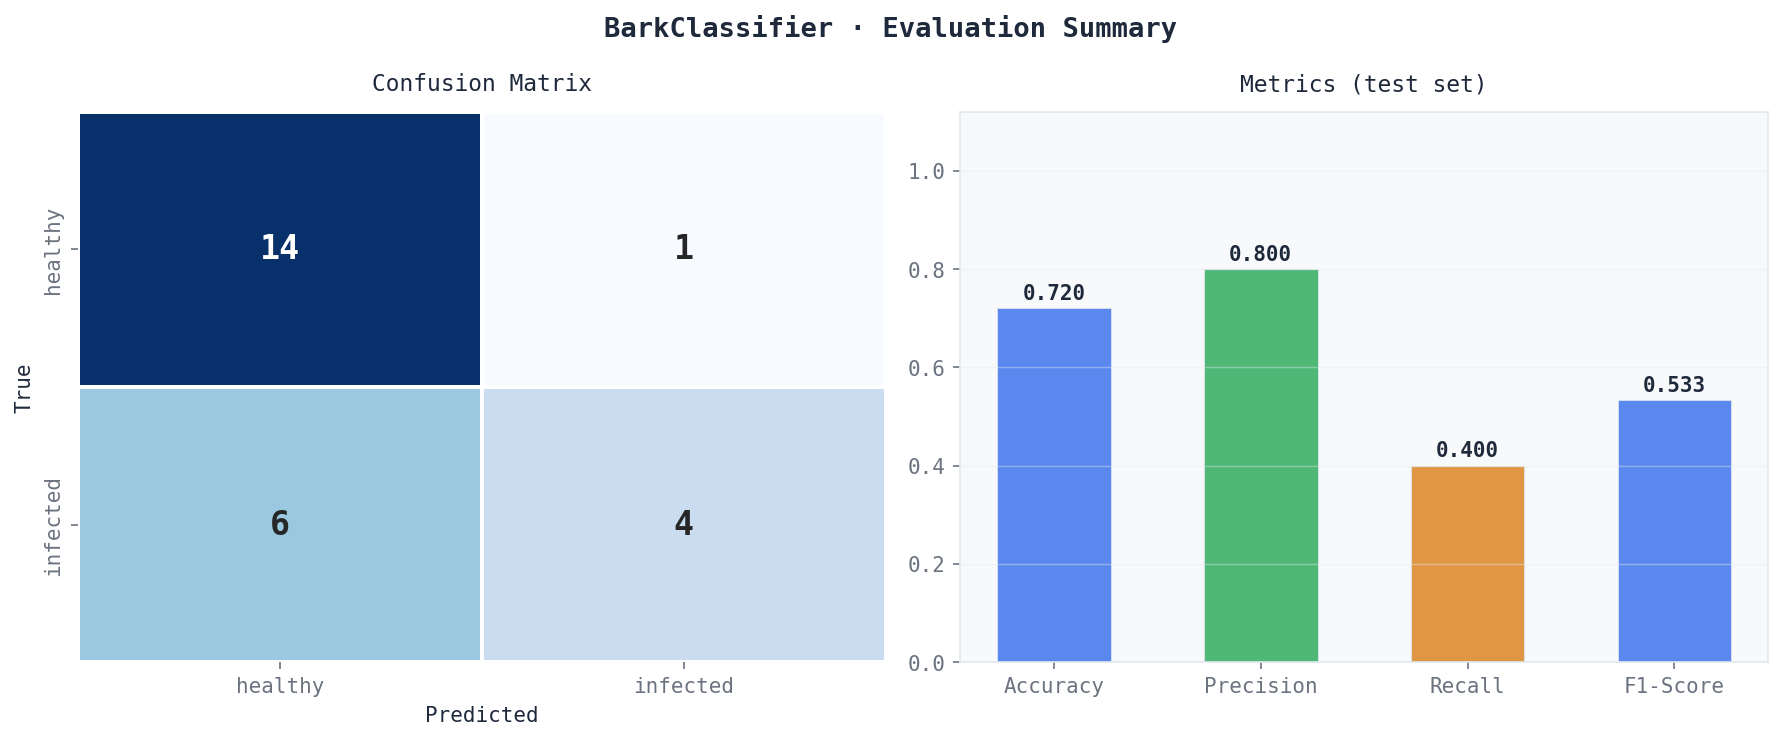
\includegraphics[width=0.8\textwidth]{images/C7/evaluation.png}
    \caption{Evaluación del modelo sobre el conjunto de validación.}
    \label{fig:evaluation}
\end{figure}

Los resultados de evaluación (Figura~\ref{fig:evaluation}) reportan una exactitud del 72\%, con una precisión del 80\% y un recall del 40\%. La precisión indica que cuando el modelo predice infestación, acierta en 4 de cada 5 casos; sin embargo, el recall bajo revela que detecta únicamente la mitad de los árboles realmente infestados. Este patrón es característico de modelos entrenados con datos insuficientes para la clase positiva: el modelo es conservador al emitir predicciones de infestación, lo que reduce los falsos positivos a costa de aumentar los falsos negativos. En el contexto de detección de plagas, mejorar el recall es prioritario, ya que un árbol infestado no detectado representa un riesgo de propagación.

\begin{figure}[H]
    \centering
    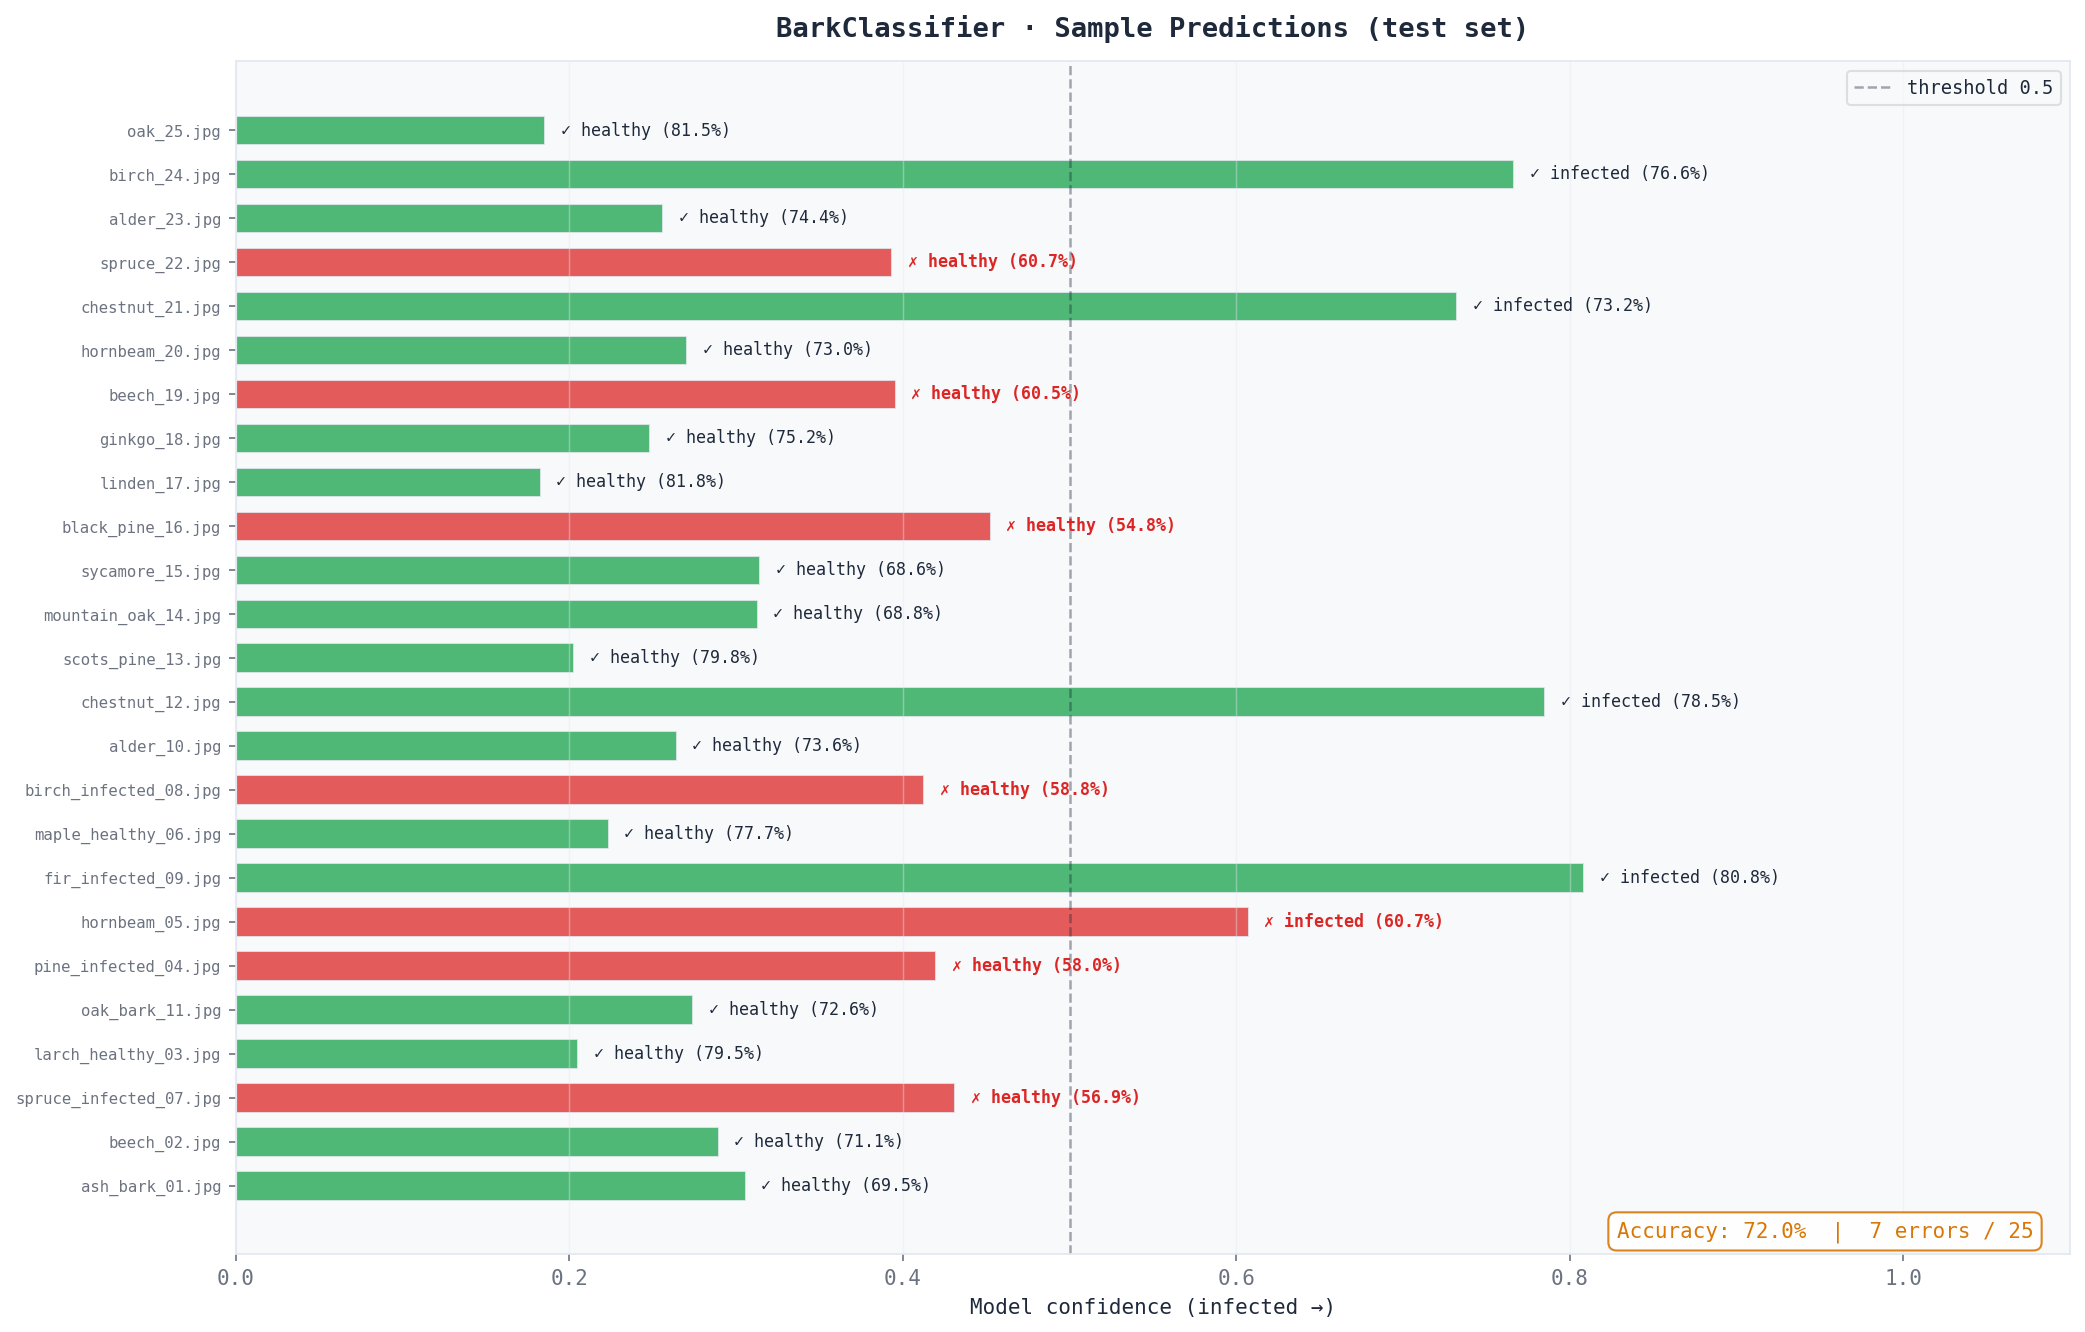
\includegraphics[width=1\textwidth]{images/C7/predictions.png}
    \caption{Predicciones sobre imágenes no vistas durante el entrenamiento.}
    \label{fig:predictions}
\end{figure}

Las predicciones sobre imágenes nuevas (Figura~\ref{fig:predictions}) confirman lo observado: el modelo opera con niveles de confianza moderados, generalmente entre el 68\% y el 85\% en los aciertos, mientras que los errores se concentran cerca del umbral de decisión (51\%--62\%), lo que indica que el modelo duda en casos ambiguos en lugar de cometer errores categóricos. De 25 muestras, 7 fueron clasificadas incorrectamente, todas con confianza baja. Este comportamiento es una señal positiva: sugiere que el modelo ha aprendido representaciones parcialmente discriminativas y que, con mayor volumen de datos, la frontera de decisión se definiría con mayor claridad.

Se estima que incrementar el conjunto de entrenamiento a entre 10,000 y 20,000 imágenes por clase permitiría al modelo mejorar su generalización y alcanzar niveles de exactitud y recall mejores.